\documentclass[tikz]{standalone}
\input{common/tikzBase}
\usetikzlibrary{}
\newsavebox{\simpleRetCheckA}
\newsavebox{\simpleRetCheckB}
\begin{document}
\begin{lrbox}{\simpleRetCheckA}
\begin{lstlisting}[language=myasm,style=smaller]
...
    call foo
    label $0xf19279bb // random ID for function foo
...
\end{lstlisting}
\end{lrbox}
\begin{lrbox}{\simpleRetCheckB}
\begin{lstlisting}[language=myasm,style=smaller]
foo: 
...
    pop %rdx          // RDX <- return address
    cmp $0xf19279bb, 2(%rdx) 
    jne CRASH
    jmp *%rdx
\end{lstlisting}
\end{lrbox}

\setSlide{1}
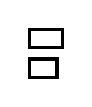
\begin{tikzpicture}
\node[font=\tt,align=left,draw,very thick] (the call) {
\usebox{\simpleRetCheckA}
};
\node[align=left,anchor=north west,draw,very thick] at ([yshift=-.1cm]the call.south west) {
\usebox{\simpleRetCheckB}
};
\end{tikzpicture}
\end{document}
